\documentclass[runningheads]{llncs}
\usepackage[utf8]{inputenc}
\usepackage{graphicx}
\usepackage[ngerman]{babel}
\usepackage{hyperref}

\title{Software-Metriken als Indikator für Sicherheitslücken}
\author{Thomas Buß}
\institute{
	Technische Universität Dortmund,\\
	August-Schmidt-Straße 4,\\
	44227 Dortmund, Deutschland\\
	\email{thomas.buss@tu-dortmund.de}
}
\date{\today}

\hyphenation{Da-tei-en}
\hyphenation{Quell-code-Da-tei-en}


\begin{document}
\maketitle
\begin{abstract}
The abstract should briefly summarize the contents of the paper in
150--250 words.

\keywords{Security  \and Metrics \and Vulnerabilities}
\end{abstract}

\section{Einleitung}
\label{sec:einleitung}
In diesem Abschnitt soll einen Einstieg in die Thematik gegeben werden.
Es wird zunächst auf die Problemstellung eingegangen und eine Motivation für das Forschungsthema geben.
Danach folgt die Formulierung eines praxisorientierten Ziels für die weiteren Überlegungen.

\subsection{Problemstellung}
Die heutzutage als selbstverständlich geltende Allgegenwärtigkeit von Software-gesteuerten Maschinen geht mit einem hohen Gefahrenpotential einher.
Software ist in fast jedem Aspekt unseres täglichen Lebens involviert.
Fehler oder Sicherheitslücken können daher weitreichende Folgen haben, die von Datenschutzverletzungen über finanziellen Schaden bis zur Lebensgefahr reichen.

Es ist zweifelsohne wünschenswert, derartige Fehler in Software so schnell wie möglich zu erkennen und zu beheben.
Gerade bei sicherheitsbezogenen Problemen ist die Lösung des Problems jedoch schwer:
Sicherheitsexperten, die Schwachstellen in der Software erkennen und beheben können, sind selten in jeder Firma vertreten und vergleichsweise teuer.
Auch wenn ein solcher Experte verfügbar ist, so würde die Überprüfung einer kompletten Software-Lösung eine große Zeitspanne einnehmen und ist daher nicht praktikabel.

\subsection{Zielsetzung}
Ein automatisches System zur Erkennung von potentiellen Schwachstellen wäre wünschenswert.
Dieses könnte dabei assistieren, die Arbeit von Sicherheitsexperten auf die Code-Bereiche zu fokussieren, die relevant für eine Überprüfung sind.
Dadurch könnte viel Arbeitszeit und somit auch Kosten reduziert werden.

Es stellt sich die Frage, mit welchen Mitteln ein solches System Schwachstellen erkennen könnte.
Software-Metriken stellen in diesem Kontext einen geeigneten Kandidaten dar.
Sie werden hauptsächlich für die Erfassung von Software-Qualitätsmaßen verwendet, können aber auch, wie im Verlauf der Ausarbeitung gezeigt wird, verwendet werden, um Schwachstellen in Software aufzudecken.

\section{Begriffe}
\label{sec:begriffe}
Bevor sich Hypothesen über den Zusammenhang zwischen Software-Metriken und Sicherheitslücken formulieren lassen, müssen diese beiden Begriffe zunächst erläutert werden.

\subsection{Software-Metrik}
Software-Metriken beschreiben Charakteristika eines Software-Systems mittels eines Zahlenwertes.
Speziell geht es in dieser Ausarbeitung um Metriken für ein einzelnes, abgeschlossenes Programm.
Neben diesen gibt es im sicherheitsbezogenen Kontext auch Metriken, die in einem Rechnernetzwerk erfasst werden können (siehe \cite{cheng2014}).
Zur Erfassung von Software-Metriken können statische Code-Analysewerkzeuge verwendet werden.
Software-Metriken lassen sich auf verschiedene Art und Weise in Gruppen einteilen.
Eine mögliche Gruppierung ist die Einteilung nach Code-Level- und Design-Level-Metriken.
Unter Design-Level-Metriken versteht man solche, die nach dem Entwurf der Software (beispielsweise anhand eines UML-Klassendiagramms) berechnet werden können.
Implementierungsspezifische Metriken, wie der Anzahl Code-Zeilen, bezeichnen sich als Code-Level-Metriken.
Eine andere Gruppierung ist die Einteilung nach Komplexität-, Kopplungs- und Kohäsionsmetriken.
Diese Metriken bezeichnet man auch als CCC-Metriken und werden in den folgenden Abschnitten genauer erläutert.

\subsubsection{Komplexität}
Komplexitätsmaße beschreiben, inwieweit die Komponenten eines Systems miteinander "`verflochten"' sind.
Den Begriff zu definieren fällt dabei schwer.
Es lassen sich aber Maße finden, die Eigenschaften komplexer Systeme ausdrücken.
Ein Beispiel eines solchen Maßes ist \textit{McCabe's Cyclomatic Complexity}~\cite{mccabe1976}.
Sie zählt die Anzahl der unterschiedlichen Kontrollflüsse innerhalb eines Programms.

Komplexitätsmaße als Indikatoren für Fehler zu verwenden ergibt Sinn.
Je einfacher das System zu verstehen ist, desto weniger fehleranfällig ist es.
Fehler in komplexen Systemen zu finden gestaltet sich hingegen als schwierig.

\subsubsection{Kopplung}
Kopplungsmaße beschreiben, wie sehr einzelne Komponenten voneinander abhängig sind.
Hohe Kopplung bedeutet, dass eine Änderung viele Änderungen als Folge nach sich zieht.
Der betroffene Code sollte so klein wie möglich gehalten werden.
Ein Beispiel für Kopplungsmaße ist die Anzahl der Unterklassen oder "`Number of Children (NOC)"'.
Durch Vererbung wird die Unterklasse an die Oberklasse gekoppelt.

Kopplungsmaße sind ein guter Indikator für die Wartbarkeit von Software-Systemen.
Eine Betrachtung von Kopplung für die Findung von Fehlern ergibt daher Sinn.

\subsubsection{Kohäsion}
Kohäsion beschreibt, inwieweit die Methoden und Variablen einer Klasse zueinander in Verbindung stehen.
So sollte sich eine Klasse nach dem "`Single Responsibility Principle"' nur um eine Aufgabe oder ein Konzept kümmern.
Geringe Kohäsion ist ein Anzeichen dafür, dass eine Klasse in mehrere aufgeteilt werden sollte.
Hohe Kohäsion bewirkt, dass die Klasse einfacher zu verstehen ist und erhöht die Wiederverwendbarkeit.
Ein Beispiel für ein Kohäsionsmaß ist "`Lack of cohesion of methods (LCOM)"', in dem die Anzahl der Variablen, Methoden und Methoden, die diese Variablen verwenden, miteinander verrechnet werden.

\subsection{Sicherheitslücke}
Der Begriff \emph{Sicherheit} bezeichnet mehrere Eigenschaften.
Oftmals wird bei Sicherheit nur an Vertraulichkeit gedacht, also die Verhinderung des Zugriffs auf vertraulichen Informationen durch Unbefugte.
Aber auch die Integrität der Daten und die Verfügbarkeit des Systems gehören dazu.

Eine \emph{Sicherheitslücke} ist vorhanden, wenn ein interner Defekt einer Komponente einem externen Fehlerursache die Möglichkeit bietet, eine oder mehrere Eigenschaften der Sicherheit zu verletzen~\cite{basics}.
Die externe Fehlerursache kann sich sowohl auf fehlerhafte Komponenten als auch unbefugte Personen beziehen.

Sicherheitslücken treten immer wieder in Software-Systemen auf.
Sie entstehen durch menschliche Fehler während der Entwurfs-, Entwicklungs- und Deployment-Phasen eines Systems, insbesondere, wenn eine ungünstige Architektur die Verständlichkeit einer Komponente erschwert.
Eine allumfassende Planung zum Ausschluss von Sicherheitslücken ist praktisch unmöglich.
Daher muss neben der vorangehenden Planung eines System auch während der Entwicklung überprüft werden, ob Sicherheitslücken vorliegen.

\section{Hypothesen}
\label{sec:hypothesen}
Nachdem die Begrifflichkeiten erläutert wurden, lassen sich mit deren Hilfe Hypothesen formulieren, die den Rest dieser Ausarbeitung als Leitfaden dienen sollen.
Sicherheitslücken treten auf, wenn Entwickler aufgrund der Komplexität des Systems unabsichtlich defekte Komponenten entwickeln.
Es stellt sich also die Frage, ob diese Schwächen in der Software-Architektur,
sowohl auf einer höheren, abstrakten Ebene, als auch auf einer niedrigeren, konkreten Ebene,
sich durch Metriken erkennen und somit potentiell defekte Komponenten mit Sicherheitslücken aufspüren lassen.

Viele Hypothesen sind für dieses Forschungsgebiet denkbar.
Die nachfolgenden Hypothesen sollen in dieser Ausarbeitung näher betrachtet werden.
Sie orientieren sich an der Forschung von Alves et. al (siehe \cite{alves_et_al}).

\subsection{Vorhersagbarkeit von Sicherheitslücken durch Metriken}
Die erste Hypothese lautet: "`Durch Software-Metriken lassen sich Rückschlüsse auf die Existenz von Sicherheitslücken schließen"'.
Dies ist die zentrale Hypothese der Ausarbeitung.
Wenn sie bestätigt werden kann, lassen sich durch Software-Metriken automatisierte Werkzeuge für Entwickler erstellen, die bei der Auffindung von Sicherheitslücken helfen.

\subsection{Vorhersagbarkeit von Anzahl an Sicherheitslücken}
Die zweite Hypothese lautet: "`Durch Software-Metriken lassen sich Rückschlüsse auf die Anzahl der Sicherheitslücken schließen"'.
Wenn sich die erste Hypothese bestätigen lässt, ist es zusätzlich von Vorteil, die Anzahl der Sicherheitslücken voraussagen zu können.

\subsection{Korrelation zwischen Software-Metriken}
Die dritte Hypothese lautet: "`Einige Software-Metriken korrelieren miteinander"'.
Es ist nicht bekannt, welche Software-Metriken sich besonders gut oder schlecht für die Vorhersage von Sicherheitslücken eignen.
Außerdem könnten sich Redundanzen und Widersprüche in den Vorhersagen finden.
Daher ist es naheliegend zu untersuchen, welche Menge von Software-Metriken für eine Vorhersage ausgewählt werden sollte.

\section{Erfassung der Daten und Aufbereitung}
\label{sec:erfassung}
In diesem Abschnitt wird beleuchtet, wie die für die Verifikation der Hypothesen notwendigen Daten erfasst werden können.
Gegebenenfalls müssen die Daten für eine Analyse ebenfalls vorverarbeitet werden, um einen brauchbaren Datensatz zu erhalten.
Die Qualität der zugrunde liegenden Daten bestimmt die Aussagekraft, mit der die Hypothesen verifiziert oder verworfen werden können.

Für die Analyse eignen sich Open Source Projekte,
da diese sowohl den Quellcode als auch verschiedene Issue-Tracker,
in denen Sicherheitslücken gelistet sind,
öffentlich zugänglich machen.
In den Arbeiten von Chowdhury und Zulkernine wird \emph{Mozilla Firefox} als Gegenstand der Fallstudien verwendet~\cite{chowdhury_zulkernine_2010,chowdhury_zulkernine_2009}.
Die Festlegung auf ein einziges Projekt limitiert jedoch die Aussagekraft der Studie.
Daher haben Alves et al. mehrere Projekte für ihre Studie ausgewählt~\cite{alves_et_al}: 
Mozilla Projekte (Firefox, Thunderbird und andere),
den Linux Kernel,
den \emph{Xen} Hypervisor,
den Apache Webserver \texttt{httpd} und
die GNU Bibliothek \texttt{glibc}.

Informationen über Sicherheitslücken lassen sich über sog. \emph{Security Advisories} erhalten.
Diese listen entdeckte Bugs in der Software auf, die einen sicherheitsbezogenen Kontext haben.
Ein Eintrag in einer diesem Advisories enthält Informationen über die Sicherheitslücke, eine Bewertung der Schwere dieser Lücke und einen Link zu dem entsprechenden Bug-Tracker-Eintrag.
Abbildung \ref{fig:mfsa} zeigt einen Eintrag auf der \textit{Mozilla Foundation Security Advisories}\footnote{\url{https://www.mozilla.org/en-US/security/advisories/}} Webseite, die von verschiedenen Forschern verwendet werden~\cite{alves_et_al,chowdhury_zulkernine_2010}.
Für viele andere Projekte existieren ebenfalls Security Advisories.
\begin{figure}
	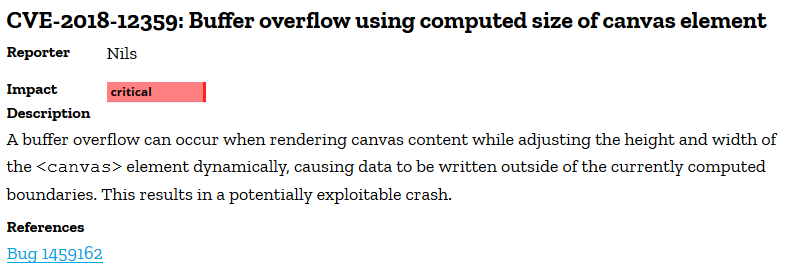
\includegraphics[width=\textwidth]{img/mfsa_example.png}
	\caption{Beispieleintrag auf der \textit{Mozilla Foundation Security Advisories} Webseite}
	\label{fig:mfsa}
\end{figure}

Für die statische Codeanalyse wird der Quellcode in zwei Versionen benötigt, nämlich vor und nach dem Beheben einer Sicherheitslücke.
Auf beiden Version wird die Codeanalyse ausgeführt, um die Metriken zu berechnen.
Durch die Unterschiede in den Metriken lässt sich ermitteln, was das Beheben einer Sicherheitslücke in den Metriken bewirkt.

Über die Security Advisories und den Bug Trackern lassen sich die Versionen bzw. Commits finden, in denen die Sicherheitslücken geschlossen wurden.
Dafür werden Parser-Programme verwendet, die die aufgelisteten Sicherheitslücken durchsuchen und die Referenzen auf die Versionen bzw. Commits der Behebungen ermitteln~\cite{alves_et_al,chowdhury_zulkernine_2009}.
Da die Einträge nicht immer konsistent gehalten werden, erschwert dies die Arbeit der Parser.
Alves et al. konnten daher nur 55 \% der Einträge in den untersuchten Projekten verarbeiten~\cite{alves_et_al}.
Das lässt viele Sicherheitslücken aus und mindert daher die Menge geeigneter Daten.

Ist die Version einer Software gefunden, in der eine Sicherheitslücke geschlossen wurde, kann die statische Codeanalyse durchgeführt werden.
Für einen Vergleich der Metriken muss eine andere Version ebenfalls analysiert werden, bestenfalls der Commit, der direkt vor dem Schließen der Lücke steht.
Alves et al. nehmen hierfür den Commit, der sich direkt davor in der Historie verwendet.
Es besteht allerdings die Möglichkeit, dass eine Lücke in mehreren Commits bearbeitet wird.
Der letzte Commit könnte beispielsweise nur "`Schönheitskorrekturen"' beinhalten, die keinerlei Auswirkungen auf die Metriken haben.
Ebenso ist es denkbar, dass der Hauptzweig kurz vor Schließung der Sicherheitslücke gemerged wurde.
Dann enthält dieser Commit potentiell sehr viele Änderungen, die nicht in Verbindung mit der Sicherheitslücke stehen.
Damit wären die Metriken sehr verschieden.
Chowdhury und Zulkernine verwenden für ihre Studie Release-Versionen von Mozilla Firefox.
Diese Herangehensweise ist kritisch zu betrachten, da damit die Ergebnisse der Codeanalyse verfälscht werden können.
Release-Versionen beinhalten in der Regel viele Änderungen, sodass die Metriken keinen Bezug zur Sicherheitslücke haben.

Die Erfassung der Metriken kann auf verschiedenen Ebenen erfolgen, beispielsweise auf Klassenebene oder Funktionsebene.
Eine einfache Art stellt die Dateiebene dar.
Sie ist universell für alle Arten von Software-Systemen.
Für andere Ebenen ist es notwendig, die Dateien zu parsen.
Unterschiedliche Sprachen bieten auch unterschiedliche Gruppierungsmechanismen an.
In C gibt es beispielsweise keine Klassen.
Deshalb wird in der Arbeit von Alves et al. bei den Projekten, die in C geschrieben wurden, \texttt{Structs} und \texttt{Unions} wie Klassen in C++ behandelt.

Bei Verwendung der Dateiebene für die Erfassung der Metriken muss bedacht werden, wie sich der Wert einer Datei aus den analysierten Elementen zusammensetzt.
Befinden sich in einer Datei beispielsweise zwei Klassen mit unterschiedlichen Metrik-Werten, müssen diese Werte zusammengefasst werden.
Eine Möglichkeit die Werte zusammenzufassen ist das arithmetische Mittel zu berechnen~\cite{chowdhury_zulkernine_2009}.
Alternativ dazu kann man auch das Maximum bilden.
Analoges gilt bei der Erfassung von Metriken auf Klassenebene unter Einbeziehung der jeweiligen Methoden der Klasse.

Die Wahl des Programms zur Berechnung der Metriken hängt von der Analyse ab, die anschließend mit den Metriken vorgenommen werden soll.
Nicht jedes Programm kann alle gewünschten Metriken berechnen und eigene Implementationen sind zeitaufwendig.
In den Studien von Alves et al. und Chowdhury und Zulkernine kam dafür das Tool \emph{Understand}\footnote{Understand Webseite: \url{https://scitools.com/features/}} zum Einsatz~\cite{alves_et_al,chowdhury_zulkernine_2009}.
Damit konnten alle benötigten Metriken für die Analyse erfasst werden, wenn auch einige wünschenswerte Metriken fehlten.

\section{Analyse}
\label{sec:analyse}
Nachdem ein geeigneter Datensatz erfasst wurde, können die Daten analysiert werden.
Für die Analyse gibt es zwei wesentliche Herangehensweisen: Korrelationsmaße und Klassifikatoren.
Zuvor sollte festgelegt werden, welche Metriken für die Analyse verwendet werden sollen.
%TODO Medeiros et. al versuchen, die besten Metriken herauszufinden!
% Informational approach (Wo fließen Daten hin?) vs. structual approach (Wer ruft wen auf?)

\subsection{Wahl der Metriken}
Die Auswahl der Metriken ist vielfältig.
In \cite{alves_et_al} werden insgesamt 27 Metriken für Funktionen berechnet.
Einige davon sind CCC-Metriken\footnote{Die Metriken sind jedoch nicht in die Komplexität, Kopplung und Kohäsion eingeteilt.}, andere beziehen sich auf die Anzahl der Codezeilen oder auf das Verhältnis von Quellcode-Kommentaren zu Codezeilen.
In der Studie aus \cite{chowdhury_zulkernine_2009} werden 21 Metriken berechnet.
Die Forscher teilen dabei die Metriken sowohl in die CCC-Klassen, als auch in Code-Level und Design-Level ein.
Unter Design-Level-Metriken versteht man dabei solche, die nach dem Entwurf der Software (beispielsweise anhand eines UML-Klassendiagramms) berechnet werden können.
Implementierungsspezifische Metriken wie die Anzahl Code-Zeilen bezeichnen sich als Code-Level-Metriken.
Abbildung \ref{fig:chowdhury_metrics} zeigt einen Ausschnitt aus \cite{chowdhury_zulkernine_2010}.
Zu sehen sind die Bezeichnung und englische Beschreibungen für die Komplexitätsmetriken.
\begin{figure}
	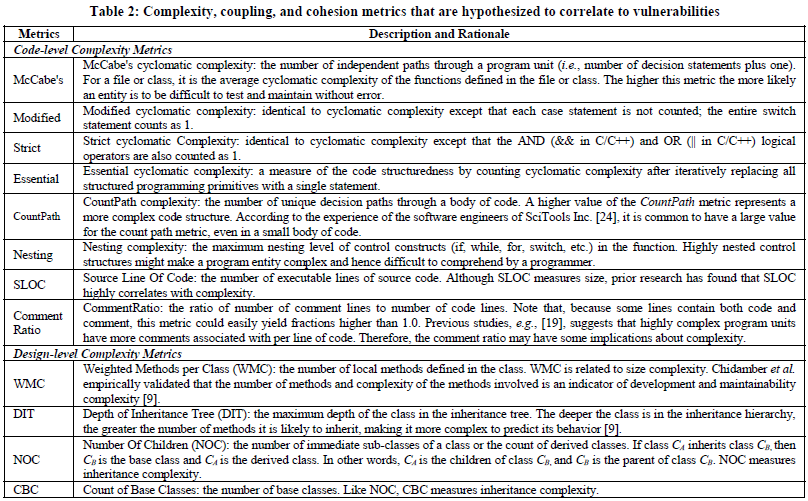
\includegraphics[width=\textwidth]{img/chowdhury_metrics.png}
	\caption{Auszug aus \cite{chowdhury_zulkernine_2010}; Tabelle mit den verwendeten Metriken.}
	\label{fig:chowdhury_metrics}
\end{figure}

\subsection{Korrelationsmaße}
Zur Überprüfung der Hypothesen eigen sich Korrelationsmaße.
Die Behebung einer Sicherheitslücke müsste eine Verbesserung der CCC-Metriken nach sich ziehen.
Ein mögliches Maß für die Korrelation ist Spearmans Rangkorrelationskoeffizient~\cite{alves_et_al,chowdhury_zulkernine_2010}, da dieses keine Annahmen zur Verteilung macht.
Der Spearman Korrelationskoeffizient (kurz: die Korrelation) ist ein Wert zwischen -1 und +1, wobei -1 eine stark negative und +1 eine stark positive Korrelation ausdrückt.
Die Signifikanz der Korrelation wird mit dem p-Wert ausgerückt.
Ein p-Wert kleiner 0.05 wird als statistisch signifikant gewertet.
Weitere Techniken, die beispielsweise in \cite{alves_et_al} verwendet werden, sind der zweiseitige t-Test, Konfidenzintervalle und der Wilcoxon Rangsummentest.
\begin{figure}
	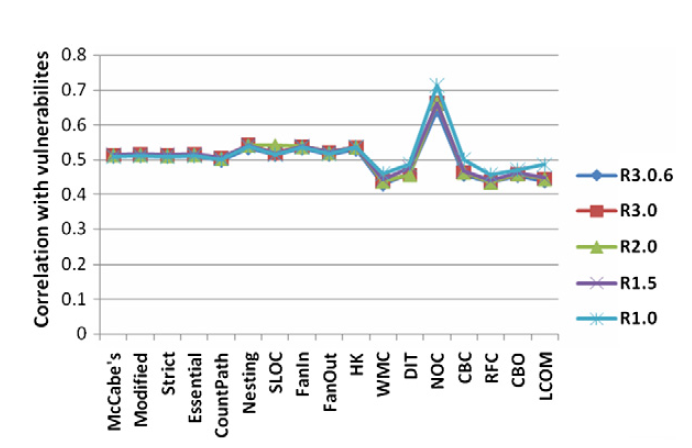
\includegraphics[width=\textwidth]{img/vulnerability_correlations.png}
	\caption{Korrelationen mit Sicherheitslücken zu verschiedenen Metriken}
	\label{fig:correlations}
\end{figure}
Abbildung \ref{fig:correlations} aus \cite{chowdhury_zulkernine_2009} zeigt die Korrelation mit Sicherheitslücken zu verschiedenen Metriken.
Die Linien zeigen verschiedene Release-Versionen von Mozilla Firefox.
Es lässt sich erkenne, dass die Korrelationsmuster über Versionen hinweg konsistent sind\cite{chowdhury_zulkernine_2009}.

\subsection{Klassifikatoren}
Mithilfe der Metriken lassen sich auch Klassifikatoren (englisch: \emph{predictors}) erstellen.
Dieser Ansatz wird in \cite{chowdhury_zulkernine_2009} verwendet, um ein Framework für die Vorhersage von Sicherheitslücken zu entwickeln.
Abbildung \ref{fig:framework} zeigt die Architektur dieses Frameworks.
\begin{figure}
	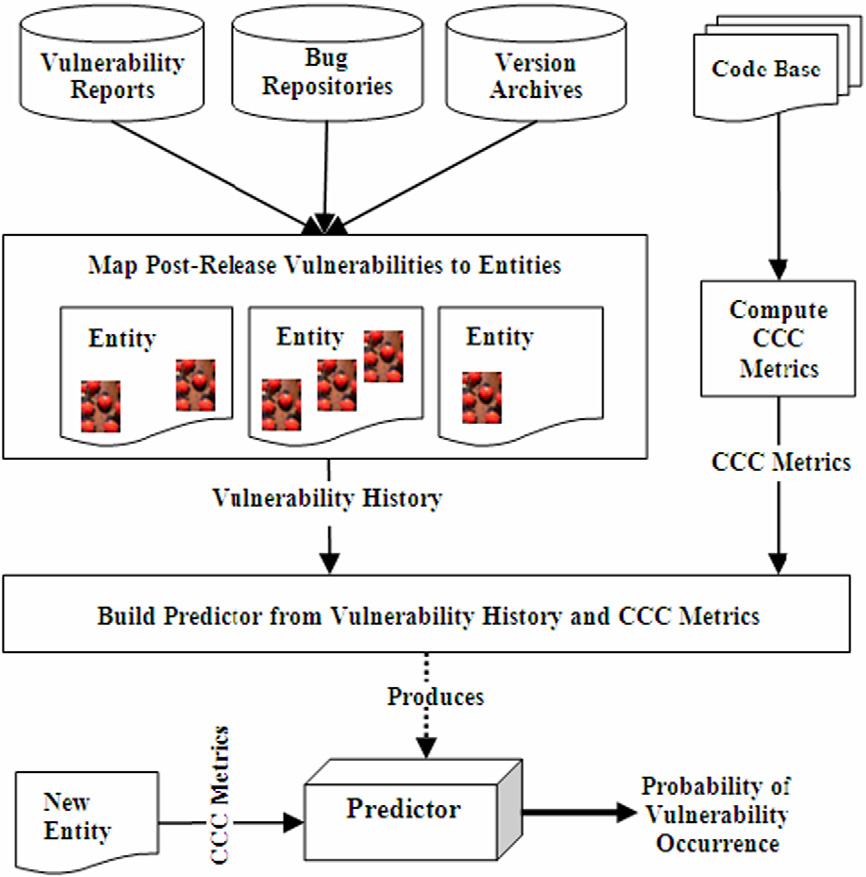
\includegraphics[width=\textwidth]{img/framework.png}
	\caption{Framework für die Vorhersage von Sicherheitslücken aus \cite{chowdhury_zulkernine_2009}}
	\label{fig:framework}
\end{figure}
Die Herangehensweise unterscheidet sich dahingehend von der Berechnung der Korrelationen, dass die in anderen Studien festgestellte Korrelation der Metriken mit Sicherheitslücken nicht verwendet wurde, um Vorhersagen zu erstellen.

Das Problem wird als Klassifizierungsproblem auf Dateiebene aufgefasst:
Entweder eine Datei ist anfällig für Sicherheitslücken oder nicht.
Für die Klassifikatoren kommen verschiedene Techniken in Frage.
Beispiele sind \emph{C4.5 Entscheidungsbäume}\cite{decision_trees}, die Weiterentwicklung \emph{Random Forests} und der \emph{Bayes-Klassifikator}.
Die in \cite{chowdhury_zulkernine_2009} für die Generierung der Klassifikatoren verwendete Bibliothek ist \emph{Waikato Environment for Knowledge Analysis (WEKA)}\footnote{WEKA Webseite: \url{https://www.cs.waikato.ac.nz/ml/weka/}} der Universität von Waikato, Neuseeland.
Sie ist Open Source und in Java implementiert, sodass sie einfach und vielseitig eingesetzt werden kann.

Für die Generierung ist es notwendig, einen ausbalancierten Datensatz zu verwenden, um einseitige Klassifikatoren auszuschließen.
Anschließend können die Klassifikatoren generiert werden.
Ein Verfahren dafür ist \emph{Cross Validation}\cite{chowdhury_zulkernine_2009}.
Der Datensatz wird in 10 "`Bins"' aufgeteilt, wovon 9 zum Trainieren des Klassifikators und einer zum Testen der Vorhersagen benutzt werden.
Dieser Vorgang wird einige Male wiederholt.

Die generierten Klassifikatoren müssen anschließend noch auf ihre Qualität überprüft werden.
In \cite{chowdhury_zulkernine_2009} werden dafür die folgenden Maße verwendet:
\begin{equation}
	Accuracy = \frac{TP+TN}{TP+FP+TN+FN}
\end{equation}
\begin{equation}
	Recall = \frac{TP}{TP+FN}
\end{equation}
\begin{equation}
	FN rate = \frac{FN}{TP+FN}
\end{equation}
Dabei ist \emph{TP} (true positives) die Anzahl der korrekt erkannten Sicherheitslücken,
\emph{TN} (true negatives) die Anzahl der korrekt als ohne Lücke erkannten Dateien,
\emph{FP} (false positives) die Anzahl der fälschlicherweise erkannten Sicherheitslücken und
\emph{FN} (false negatives) die Anzahl der nicht erkannten Sicherheitslücken.

\section{Ergebnisse}
\label{sec:ergebnisse}
In diesem Abschnitt werden die Ergebnisse der Datenauswertung wiedergegeben und interpretiert.

\section{Fazit}
\label{sec:fazit}
Es konnte gezeigt werden, dass Software-Metriken mit Sicherheitslücken korrelieren und sich damit Codestellen mit potenziellen Sicherheitslücken erfassen lassen.
Eine verlässliche Voraussage über Anzahl der Sicherheitslücken lässt sich nicht treffen.
Die Ergebnisse sind über mehrere Versionen der gleichen Software als auch bei verschiedenen Projekten konsistent.
Für eine optimale Analyse müssen die verwendeten Metriken projektabhängig gewählt werden und sollten verschiedene Ebenen (Funktions-, Datei- und Projektebene) abdecken.
Die historische Betrachtung der Sicherheitslücken eines Projektes kann die Ergebnisse verbessern.
Dieses Wissen kann genutzt werden, um automatisierte Tools zu erstellen, die bei der Entwicklung helfen und Schwachstellen frühzeitig erkennen.

\section{Ausblick}
\label{sec:ausblick}
In den vorangegangenen Abschnitten wurden die aktuellen Forschungsergebnisse zu diesem Gebiet vorgetragen und zusammengefasst.
Zum Schluss dieser Ausarbeitung soll noch ein Ausblick über künftige Entwicklungen auf diesem Forschungsgebiet gegeben werden.

Die Verfahren zur Vorhersage und die Auswahl der verwendeten Metriken kann noch weiter optimiert werden, um bessere Vorhersagemodelle zu entwickeln.

Die Eignung von anderen Metriken für die Vorhersage von Sicherheitslücken kann weiter untersucht werden.
Bisherige Untersuchungen haben sich auf objekt-orientierte Programmiersprachen die C++ konzentriert.
Eine Ausweitung auf andere Programmiersprachen und Software-Architekturen wie service-orientierte Architekturen könnte weitere Erkenntnisse liefern\cite{chowdhury_zulkernine_2009}.

Ein Problem, welches sich bei Alves \emph{et al} \cite{alves_et_al} gezeigt hat, ist die Datenerhebung.
Lediglich 55\% der Sicherheitslücken konnten durch das verwendete Programm analysiert werden.
Zudem kommen nicht viele Projekte für die Analyse in Frage, da nur wenige Open Source Projekte Security Advisories haben\footnote{Daher haben auch viele der betrachteten Studien \emph{Mozilla Foundation Security Advisories} als Quelle der Daten verwendet}.
Ein besseres Verfahren zur Datengewinnung könnte die Präzision der Ergebnisse verbessern und repräsentativer machen.

\section*{Erklärung zur Urheberschaft}
Hiermit erkläre ich, dass ich mein Essay
eigenständig und nur mit den
angegebenen Hilfsmitteln und der
angegebenen Literatur verfasst habe.

\bibliographystyle{splncs04}
\begin{thebibliography}{8}
\bibitem{cheng2014}
Cheng, Yi et. al: Metrics of Security, Cyber Defense and Situational Awareness, Springer International Publishing (2014), S. 263--295
ISBN: 978-3-319-11391-3

\bibitem{mccabe1976}
McCabe, Thomas J.: A Complexity Measure, IEEE Transactions on Software Engineering, Vol. SE-2 No. 4, (1976)
\end{thebibliography}

\end{document}
